\part{Expression des besoins}

Étape de l’élaboration du dossier d'expression des besoins (conformément au dossier d’initialisation) : 

Le dossier d’expression des besoins contient plusieurs sous-dossiers : 
\begin{itemize}
\item Etude de l’existant, à savoir l’analyse des processus qui permettent aujourd’hui de gérer les contrats de maintenance. Le but de cette partie est donc d’avoir une vision critique de l’existant afin d’émettre un diagnostic dans l’optique de proposer une solution qui apporte une avancée par rapport à  ce qui existe déjà.
\item Dégager les processus principaux ainsi que des objets métiers.
\item Étude de l’existant.
\item Benchmarking.
\item Élaboration de la cible fonctionnelle.
\item Définition des thèmes de progrès (s’il en est).
\end{itemize}

Avant de citer les différents éléments qui permettent de gérer les contrats de maintenance chez SPIE. Nous allons décrire les activités de SPIE dans une première partie, nous nous concentrerons notamment au niveau de SPIE Sud-Est.

\section{Etude de l'existant}

\subsection{Activités de SPIE}

Rappel de l’existant au niveau de SPIE Sud-Est :

SPIE Sud-Est est structuré en 3 directions de spécialité qui dépendent de la direction générale :

\begin{itemize}
\item Génie climatique
\item Industries
\item Systèmes d’informations et transport
\end{itemize}

SPIE Sud-Est est divisé en 7 directions opérationnelles : 1 direction opérationnelle étant un découpage géographique au sein de la région SPIE Sud-Est. De manière synthétique, SPIE Sud-Est est donc présent dans les 3 grandes régions : Rhône Alpes, Auvergne, PACA et  Suisse. SPIE Sud-Est répond aux besoins de plus de 5000 clients.

%TODO : mettre juste après la carte représentant tous ces découpages géographiques.

Concevoir, Réaliser et Maintenir sont les 3 activités principales de l’entreprise, en appliquant ces services aux 3 domaines cités ci-dessus SPIE Sud-Est mènent des projets que l’on retrouve au sein de nos collectivités, par exemple :

Dans le domaine des transports, la mise en place des réseaux Cité, PrioCité, Vigicité, Sylvie,  des sytèmes permettant de gérer et de piloter les transports en communs mais aussi de réguler la circulation au sein d’une agglomération.

Dans le domaine de la gestion de l’énergie, la mise en place de Spielum, un système gérant l’éclairage public qui rend l’éclairage plus efficace et sa consommation moindre.

Dans le domaine écologique, la mise en place de projet de grande envergure de production d’énergie “verte” (photovoltaïque, hydroélectrique...).

A travers ses projets pour les réseaux de transports en commun, SPIE dispose d’une sérieuse expérience dans les domaines du SAEIV à savoir les Systèmes d’Aide à l’Exploitation et à l’Information des Voyageurs. Ceci permet donc de répondre aux attentes des utilisateurs en ce qui concerne :

\begin{itemize}
\item L’information au voyageur (embarqué, sol et internet),
\item La supervision et régulation en temps réel du réseau,
\item L’évaluation et aide à l’exploitation en temps différé.
\end{itemize}

Les systèmes d’informations, souvent nécessaire aux développements des projets que SPIE met en place sont conçus et développés au sein du département Système d’Information par 150 personnes dont 110 permanents et représentent 18 M \euro de CA. Le travail est réparti en 3 plates-formes de développement sur Lyon, Aix en Provence et Vallauris.

Ce département assure la conception, le développement, l’intégration, et la mise en service des systèmes automatisés de production, des systèmes de traitement de l’Information, des solutions d’administration des systèmes et des prestations associées (Garantie, Formation, Soutien après Vente).

sources : diapositives de JM.Berthault.

Voici une liste des filiales de SPIE Sud-Est dans les domaines du service industriel :

\begin{itemize}
\item GMS : services de maintenance et prestations mécaniques en Savoie et en Isère.
\item ACEM : services industriels en Auvergne
\item C-TRAM : services industriels dans la région lyonnaise
\item SOMELEC : services industriels en région provençale, spécialiste des services à l’industrie agroalimentaire
\item DCCS en grand dauphiné, spécialiste des systèmes de sécurité, vidéosurveillance et autres courants faibles.
\item Entreprise J. POLAUD, spécialiste des travaux extérieurs en Savoie et Nord Isère
\item PIER : services à destination des opérateurs télécom.
\item GB Analyse : spécialiste en Analyse industrielle pour l’industrie pétrochimique (maintenance et travaux clés en main dans le domaine des systèmes d’échantillonnage d’analyse.
\item ELECTROTECH : spécialiste du génie électrique en Suisse.
\end{itemize}

%source : site internet spie sud est ->
%http://www.spie.com/a-propos-de-spie2/spie-dans-le-monde1/spie-sud-est1.html#c3771

Gestion des contrats de maintenance chez SPIE
Le processus de maintenance chez SPIE (traduction de la présentation) :
Voici un diagramme représentant l'organisation de l'entreprise SPIE. SPIE est donc organisé selon deux principes principaux, à savoir les directions de proximité (comme celle de SPIE Sud-Est) couplées à des directions techniques spécifiques. Comme il est spécifié dans les documents de processus, SPIE Sud-Est va donc faire appel au Responsable d'activités maintenance afin d'avoir l'expertise technique nécessaire dans la domaine technique de la maintenance.

\begin {center}
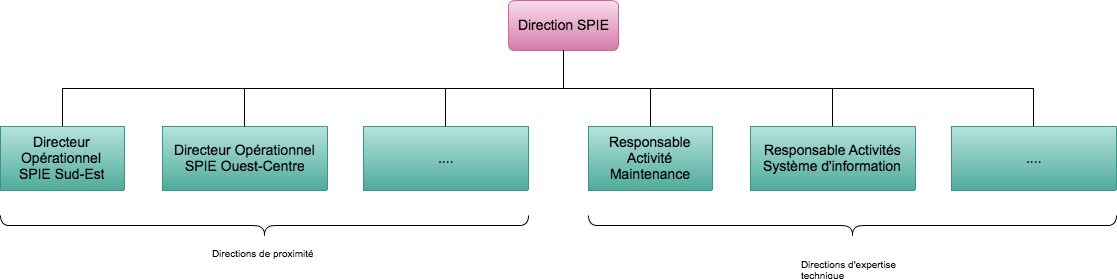
\includegraphics[width=\textwidth]{png/DiagrammeOrganisationnelSPIE.png}
\end {center}

%TODO : insérer le diagramme organisationnel de SPIE présent dans le dossier Livrable/ressource du repos git.


\paragraph{Les intervenants}

\begin{itemize}
\item Le pilote de l'offre : c'est l'acteur qui sera chargé de gérer la réponse à l'appel d'offre du client. Il ménera la validation interne de l'élaboration de l'offre et sera l'intermédiaire avec le client pour répondre aux éventuelles évolutions de spécifications du client.
\item Le responsable du contrat : c’est la personne qui assure la gestion contractuelle et le reporting, le reporting est de manière francisée l’établissement de compte rendu remis aux supérieurs et permettant d’effectuer un bilan à un moment précis de la vie du projet (à l’issue de la réalisation d’une phase ou à la remise d’un livrable par exemple).Dans le cadre de la gestion des contrats de mainteance, on nommera un responsable d'affaire (RA) chargé de suivre le projet.
\item Le Responsable d'activité maintenace : c'est la personne qui représente une direction d'expertise technique. Le RAM sera donc l'acteur vers lequel il faudra se tourner afin de statuer sur la possibilité de réalisation de telle ou telle solution technique.
\item Les techniciens de maintenance : c’est la personne (ou le groupe d’intervention) qui va intervenir sur le terrain afin d'effectuer l’acte de maintenance en tant que tel. Lui aussi est astreint à effectuer un acte de reporting auprès de son responsable afin d’informer des difficultés et/ou des solutions apportées à l’installation à maintenir. Dans le cadre de son travail d’expertise il devra informer de la nécessité d’approvisionnement en tel ou tel matériel. Exemple classique : changement d’ampoule, ajout d'équipement (de siège pour un arrêt de bus...).
\item Le contrôle de gestion : permet de valider ou non le reporting du responsable de contrat. La ressource en charge de ce contrôle de gestion ne se limite pas à la vérification pure et simple du compte rendu mais aussi d’assurer la performance économique de l’entreprise.
\end{itemize}

\paragraph{Le contrat}
Voici un schéma récapitulant les étapes clefs de la suivie du contrat de maintenance chez SPIE :

\begin {center}

\includegraphics[width=\textwidth]{png/SimplificationProcessusDeMaintenanceSPIE.png}
\end {center}

On distingue deux modes de fonctionnement pour l’établissement du contrat de maintenance :

\begin{itemize}
\item Partie forfaitaire : SPIE fournit une sorte de pack de maintenance, qui prévoit un éventail d’actes compris dans le forfait. Un document répertorie donc les choses pour lesquelles le client est couvert. Les tarifs sont fixés à partir des spécificités de chaque contrat. On admet ainsi que plus la couverture est importante, plus le prix du contrat sera élevé. 
\item Partie bon de commande : cette partie permet de répondre aux interventions exceptionnelles qui peuvent avoir lieu suite à des évènement tels que du vandalisme ou encore des accidents (de la circulation, comportement dangereux de l’utilisateur...). De même, si le client désire des évolutions non prévues dans le contrat, SPIE lui fait une proposition chiffrée pour ce genre d’intervention.
\end{itemize}

%Commentaire des schémas pour le processus de gestion des contrats de maintenance et service: http://moodle.insa-lyon.fr/file.php/108/EXISTANT_SPIE/Processus_de_maintenance_SPIE.pdf

\begin{itemize}
\item Opportunité de contrat de service
\item Offre et revue d’offre (X)
\item Négociation client 
\item Revue de commande (Q)
\item Lancement des prestations de service et travaux (Y)
\item Exécution des prestations et gestion (Y) ( coupé en 2 en fait)
\item Évolution du contrat (X)
\item Solde de l’affaire et du contrat (Y)
\item Fin de processus affaire Maintenance et Services
\end{itemize}

\subsection{Offre et revue d’offre}

Ce sous-processus peut débuter suite à un processus commercial. Le processus commercial peut consister en une prospection chez des clients ciblés et susceptibles d’être intéressés par la mise en place d’un contrat de maintenance. Ceci suppose donc que SPIE n’ait pas forcément conçu et réalisé le système qu’il va maintenir. L’offre/revue d’offre peut de même débuter  un processus travaux. Ici, la contraction d’un contrat de maintenance par un client est la suite logique de la réalisation d’un projet. Après avoir réalisé un projet complexe, SPIE propose à son client le contrat de maintenance qui fera office de “garantie payante” sur le système qui a été développé.

La réponse à un appel d’offre donne lieux à une opportunité de contrat de service. Le RA (Responsable d’affaire) et le RAM (Responsable d’activité maintenance) décident suivant les données clients, le climat concurrentiel, les opportunités de clients si une étude sera faite ou non, avec la participation du DO (Directeur Operationnel) et du COM (Commercial). Dans tous les cas, un PO (Pilote de l’offre) est désigné.

Si la réponse est négative, une confirmation de non-réponse est envoyée au client sous la forme d’un courrier type, sous la responsabilité du PO.

Si la réponse est positive, une collecte de données est effectuée en respectant une liste de données minimales à détenir suivant une liste type de données. Ces données sont ensuite analysées et donnent lieu à un rapport d’analyse des risques (juridique, technique, commercial, financier, environnemental...)  fait par les acteurs ayant les compétences requises ( MAR , Ressources Humaines, Service Moyens, Service Achats, Service Juridique,Direction QSE). Cette analyse de risques et de faisabilité permet de donner une réponse au client sur le futur de l’offre.

Après une réponse positive (SPIE Sud-Est va donc répondre à l’opportunité d’offre) , il y a d’abord une partie administrative pour initialiser le processus d’offre, qui va permettre d’enregistrer le dossier d’étude. Le dossier de réponses sera fait conformément au règlement de consultation.

Il faut ensuite donner des propositions de solutions chiffrées sous forme de fiches de calcul des déboursés et de fiches devis, en se basant sur les coûts induits lors de la réalisation de tel ou tel processus de maintenance (utilisation des contrats chiffrés précédemment).

Après prise de décision de la part du RAM/DO/RA, une solution est sélectionnée et son prix est validé, la fiche du devis retenu est alors signée.

L’offre est rédigée, avec entre autre la définition des conditions générales de vente de prestations de service. Elle est ensuite validée en interne par le DO, le RAM, le RA et le COM, (toujours sous la responsabilité du PO), avant d’être transmise dans les délais au client avec un courrier d’accompagnement. Une preuve d’envoi de cette offre est conservée.

\subsection{Négociation client}

Après la réception de l’offre par le client, celui-ci renvoie ses impressions et les modifications qu’il désire apporter à l’offre proposée par SPIE. Il se peut que certains points doivent être éclaircit afin que la maîtrise d’oeuvre et la maîtrise d’ouvrage aient la même idée du projet final.

\subsection{Revue de commande}

A l’issue de la phase de négociation avec le client, l’offre est dite validée, la commande est donc enregistrée dans le SI. Commence alors la phase de diffusion de la commande, celle-ci va alors être transmise aux différents services de SPIE Sud-Est afin d’en informer les acteurs principaux. Puisque la commande est lancée, on décide d’y assigner un PO ou pilote de l’offre chargé de mener la mise en place de la prestation de services. On convoque ensuite une commission de revue de commande permettant de chiffrer les écarts entre l’offre originale proposée par SPIE et les modifications apportées par le client. Cette phase permet de matérialiser l’offre en une commande précise qui cette fois répond aux attentes du client. Cette commande alors validée par SPIE Sud Est est alors re-soumise au client afin qu’il puisse y apporter d’ultimes modifications. Ce retour chez le client permet une fois de plus de préciser les exigences du client vis à vis du contrat de maintenance en lui même. Lorsque cette commande est validée par le client est par SPIE-Sud Est, le contrat est référencé et la prestation de service est prête à être lancée.

\subsection{Lancement des prestations de service et travaux}

Lors du lancement des prestations de service, il s’agit en premier lieu de considérer la commande, sa revue de commande, et le dossier contractuel d’étude. Via l’identification exhaustive des commandes acceptées, en puisant dans les spécifications client connues, et à l’aide des données internes récoltées auprès du QSE, de la gestion, et des ressources humaines, l’on passe de main entre la partie amont de la réalisation et la partie réalisation effectuée, en vue de prendre en compte le dossier complet, ce faisant créant le dossier d’affaires.

Le dossier complet permettra alors l’analyse des exigences et des besoins. L’analyse réalisée guide au dossier de synthèse des exigences contractuelles, faute de quoi il n’est possible de lister les ressources à mobiliser.

À son tour, l’analyse réalisée est le moteur d’une identification et d’une nomination des acteurs qui sera représentée dans un organigramme dont on ne dit pas quel acteur valide. L’organigramme contractuel ainsi créé viendra se rajouter au dossier de synthèse des exigences contractuelles et à la liste des ressources à mobiliser. La réunion de lancement sert ensuite de détonateur au travail sur les prestations de service, ce dont on rend compte par l’établissement d’un plan d’action par acteur et d’une analyse de risque prévisionnelle et provisoire.

Les exigences relatives au planning précédemment effectué et joint au compte-rendu de lancement, établissent une mobilisation des ressources disponibles et une organisation opérationnelle ce qui permet de  jauger la conformité des habilitations et  des formations requises.

Il s’agira ensuite de concevoir les procédures consignées dans des documents opérationnels, bâtis à partir du dossier de synthèse et des spécifications que le client fournit. Une fois compilées, ces données décrivent les procédures de prise en charge, le plan de maintenance initial, le plan d’assurance qualité et le plan de prévention en fonction des besoins exprimés.

Par les exigences contractuelles et par les règles de la filiale, les systèmes de gestion financière et technique sont initialisés. Le compte est alors ouvert, les supra-services sont exploités, ainsi que le système informatisé de gestion technique.

Afin d’établir un rapport d’état des lieux qui tienne compte des installations, des documents, des fournitures et des rechanges, ainsi que de l’organisation et des garanties, l’on traite alors les documents opérationnels mis au point précédemment.

Le rapport d’état des lieux une fois complété, combiné avec le dossier contractuel, permet de prendre en charge l’état des installations, le matériel et la logistique. Le PV de prise en charge ainsi créé garantie une exonération des responsabilités selon l’analyse de risque et le PAQ. Cette situation solidifie alors les fondations d’une situation initiale connue et maîtrisée, prête à une réalisation concrète.


\subsection{Réalisation des prestations de maintenance}

A la lecture du cahier des charges des travaux client, la décision est prise de donner suite, ou non, à la réalisation de prestation de maintenance. Si l’on donne suite, une analyse des travaux induits entraîne, s’ils sont faibles, une transmission des dossiers à l’entité travaux. Sinon, le contrat peut induire les modalités d’exécution des travaux induits, auquel cas il s’agit de chiffrer, valider, et d’envoyer un devis suivant les clauses contractuelles, avant réception et validation des ordres de service ou des commandes orales.

Si les dossiers sont directement transmis à l’entité travaux, le devis est envoyé directement après chiffrage et validation. A la réception de la commande, le processus rejoint celui que l’on étudiait précédemment.

L’on prépare alors les travaux, en fonction du cahier des charges, et le responsable d’exécution reçoit les consignes d’exécution. L’exécution des prestations subséquente entraîne une mise à jour des documents d’exécution. Le client peut alors signer, et la facture est déclenchée auprès du service Marché. On gère alors la garantie.

\subsection{Évolution du contrat}

Suite à la réalisation, après analyse du tableau de bord de l’affaire et des activités, des données comptables et également en fonction de l’orientation client et de l’orientation interne, la décision de renouveler ou non l’affaire sous sa forme initiale ou sous une autre forme est prise par le client, le DO, le RA, la QSE, le JUR, le ROC, sous la responsabilité du RAM.

\subsection{Solde de l’affaire et du contrat}

Le processus de gestions se termine par le solde de l’affaire et du contrat, qui consiste d’abord en une revue de fin d’affaire. Ensuite les prestations et les travaux sont soldés.

\subsection{Fin de processus affaire maintenance et service}

\subsection{Application utilisé chez SPIE}

Plusieurs applications sont utilisées pour la gestion des contrats. Il existe quatre logiciels dans la suite de SPIE pour organiser un nouveau contrat :

\begin{itemize}
\item RHI/Ndf (gestion des heures) : ce logiciel permet de prévoir et de suivre les heures et les frais correspondant à une intervention.
\item ADA/ADM (achat/moyen) : cette application permet la commande au fournisseur de tous les éléments nécessaire à une interventions.
\item ADV (administration des ventes) : lie la commande à un contrat. Permet de contrôler l’état de chaque contrat.
\item SUPRA (gestion des affaires) : création des nouveaux contrats de maintenance
\end{itemize}

\paragraph{Titre à mettre}

\begin{itemize}
\item L’objectif : l’amélioration du processus par un meilleur suivi
\item La main d’œuvre et les fournitures hors forfait
\item Les indicateurs de performance 
\item Organisationnelle : nombre d’interventions, durée (GTI, GTR), profil des intervenants,…
\item Technique : nature des travaux, moyens immobilisés, indisponibilité des installations,  …
\item Économique : volume, marge, travaux induits (devis réalisés, …)
\item Les retours d’expérience
\item Base de connaissance /métier /type de contrat
\item Identification des risques techniques/financiers/organisationnel
\end{itemize}

On distingue la gestion des contrats de maintenance de la gestion des contrats de services, description des deux mais on se focalise sur les contrats de maintenance :

\begin{itemize}
\item La gestion des contrats de maintenance se focalise sur la correction et la prévention systématique et prévisionnelle des travaux. Elle regroupe souvent aussi des fonctionnalités ouvertes à des utilisateurs au-delà du service de maintenance, comme les demandes d’interventions permettant aux personnes autorisées de signaler une anomalie à prendre en compte dans la maintenance.
\item La gestion des contrats de service s’occupe de maintenir ou rétablir un bien dans un état spécifié afin que celui-ci soit en mesure d’assurer un service déterminé.
\end{itemize}




\section{Benchmarking}


\section{Elaboration de la cible fonctionnelle}
Dans l'ensemble des processus de gestion des contrats de maintenance, nous avons mis en avant des entités organisationnelles précisent qui interviennent chacune à leur façon dans l'évolution du contrat.

\subsection{Definition du Modele d'Activité} 

\begin{itemize}
\item Gérer l'appel d'offre : étude de l'appel d'offre en interne. Cette étape est dirigée par le pilote de l'offre elle va donc permettre de proposer l'ébauche de la solution que SPIE peut apporter au client en terme de contrats de maintenance.
\item Gérer la commande : lorsque l'appel d'offre a été validé et que le client a parfaitement définit ses besoins au niveau du contrat de maintenance, SPIE est à même de lancer la \og commande \fg du contrat de maintenance. L'équipe de travail examinera donc les ressources humaines et matérielles à mettre en place pour honorer le contrat suivant les exigences formulées du client.
\item Gérer l'activité de maintenance : le responsable d'activité maintenance (RAM) au sein de SPIE garde un oeil sur l'avancée de la maintenance. Le RAM peut donc adapter la manière dont les techniciens vont intervenir sur les zones à maintenir afin de respecter les processus de maintenance definit par SPIE. Le service RH organisera la répartition des ressources humaines (technicien) qui seront en charge de l'intervention direct sur site.
\item Gérer la prestation de service : c'est l'activité du responsable d'affaire d'évaluer le déroulement du contrat. Le RA capitalise donc les informations venant de tous les acteurs du contrat de maintenance. En synthétisant toutes ces informations (reporting) et en gardant en tête les risques et les échéances il doit être capable de determiner les perspectives d'évolution du contrat.
\item Gérer l'évolution du contrat : en fonction du déroulement de la prestation de service mais aussi de la réalisation éventuelle de certains risques (surcoût, retard…). Les acteurs clefs du projet (RAM, RA, service financier) vont faire évoluer le projet. Par exemple si la prestation se passe bien il pourra être proposé au client d'étendre ce contrat de maintenance à d'autres de ces installations. Si la prestation de service sort du cadre établi lors de l'appel d'offre on établira alors des avenants.
\item Gérer la facturation : à l'issue de chaque phase clef du projet il faudra formaliser les procédures de recettes. 
\end{itemize}

Voici un modèle d'activité synthétique pour la gestion des contrats de maintenance chez SPIE :

\begin {center}
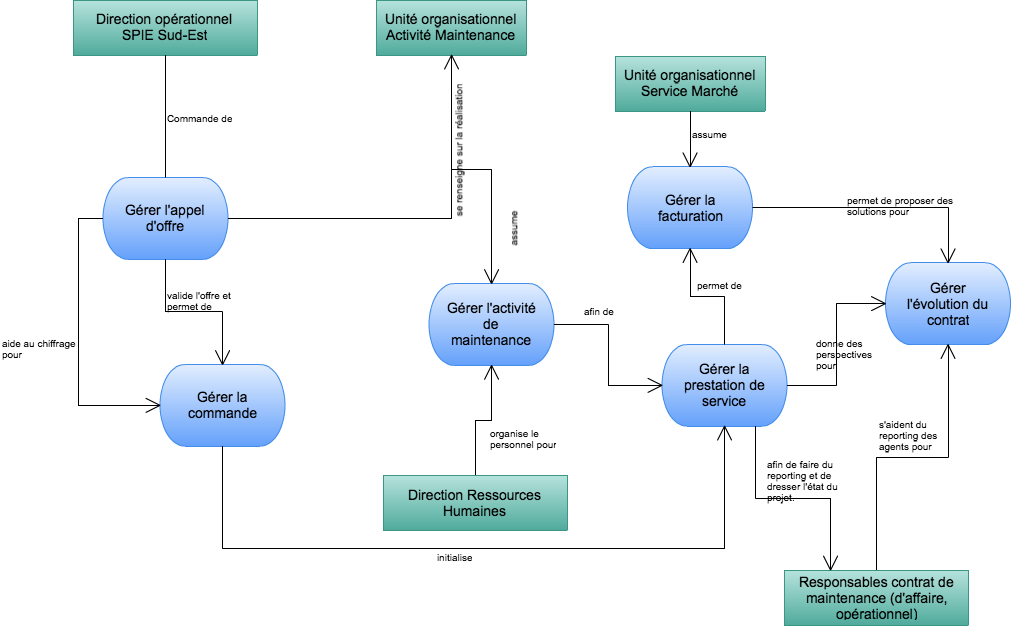
\includegraphics[width=\textwidth]{png/DiagrammeModeleActivite.png}
\end {center}

\subsection{Modèle Conceptuel des traitement} 
Vis à vis des documents fournis par SPIE, nous disposons déjà de descriptions formalisées des processus métier dans le cadre de la gestion des contrats de maintenance chez SPIE. Il nous semble donc inutile de retraduire ces processus déjà assez précis.

Il est cependant possible d'éffectuer des critiques sur la manière dont les processus s'imbriquent :

\begin{itemize}
\item Le reporting du technicien de maintenance n'est, selon nous, pas assez détaillé. En effet, il serait fortement intéressant de plus faire participer le techniciens à la rédaction, brève bien entendu, d'un rapport d'intervention qui serait concilié au sein du SI afin que son diagnostic puisse être réutilisé. Dans la même idée il serait intéressant d'affilier un technicien (ou groupe de technicien) toujours au même chantier de maintenance. Cette tactique permet ainsi au technicien de connaître parfaitement son domaine d'intervention et ainsi de minimiser le coût humain.
\item Enrichir le SI de rapports d'interventions permettrai de capitaliser et de gagner de l'expérience dans le domaine de l'expertise, un des domaines phare de SPIE.
\item Formaliser les éventuels problèmes juridiques. Un contrat avorte souvent du fait de l'incompréhension entre la MOA et la MOE. Dans les diagrammes de processus qui nous sont fournis il pourrait être pertinent d'ajouter un processus gestion des contentieux. De même, ce processus pourrait permettre d'enrichir le SI en expérience sur le déroulement des contrats.

\end{itemize}


\subsection{Diagramme de cas d'utilisation}
Il est cependant utile d'établir des diagrammes de cas d'utilisation afin de définir avec plus de précisions les notions présentes dans le modèle d'activité. Voici donc les diagrammes de cas d'utilisation correspondant à chacunes des étapes clefs de la gestion des contrats de maintenance chez SPIE.

\begin {center}
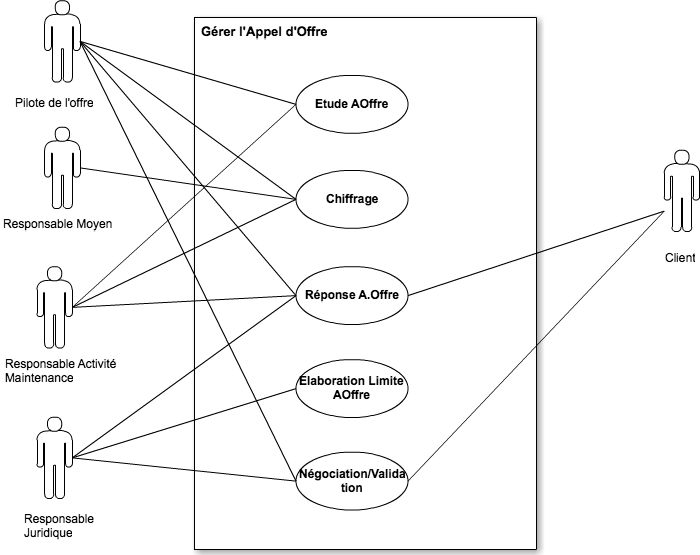
\includegraphics[width=\textwidth]{png/DCUAppelOffre.png}
\end {center}

\begin {center}
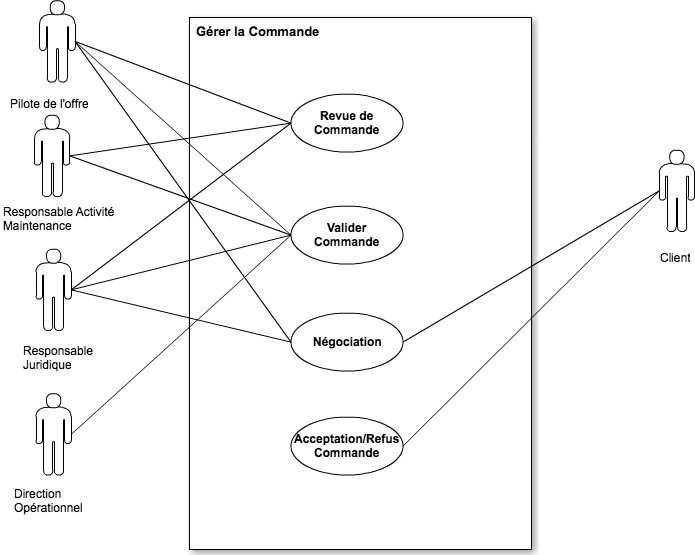
\includegraphics[width=\textwidth]{png/DCUGererCommande.png}
\end {center}

\begin {center}
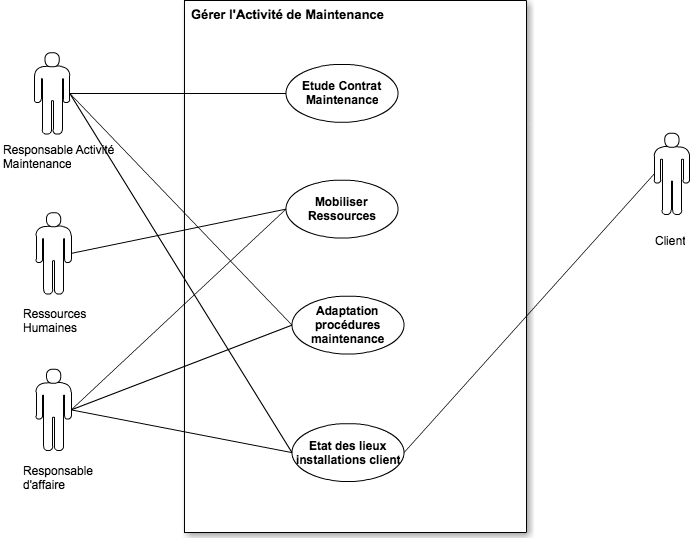
\includegraphics[width=\textwidth]{png/DCUGererActiMaintenance.png}
\end {center}

\begin {center}
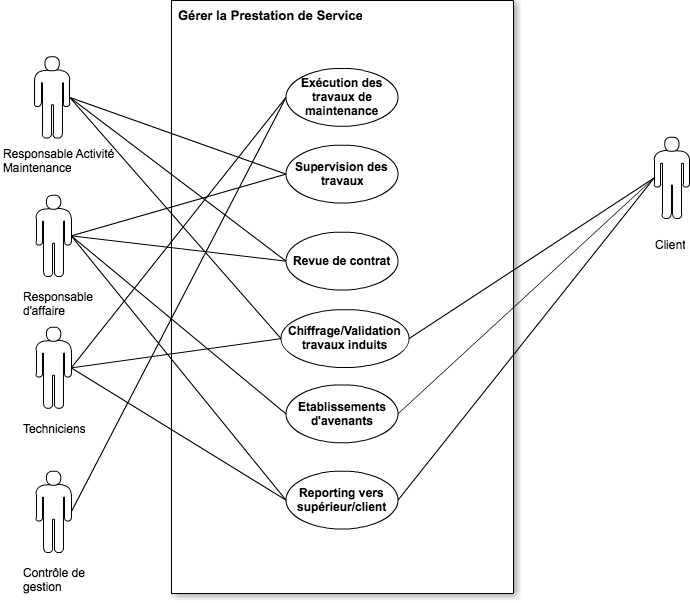
\includegraphics[width=\textwidth]{png/DCUGererPrestationService.png}
\end {center}

\begin {center}
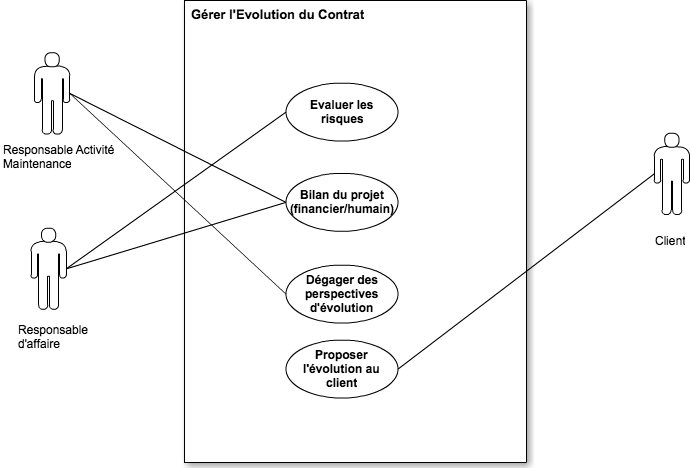
\includegraphics[width=\textwidth]{png/DCUGererEvolutionContrat.png}
\end {center}

\begin {center}
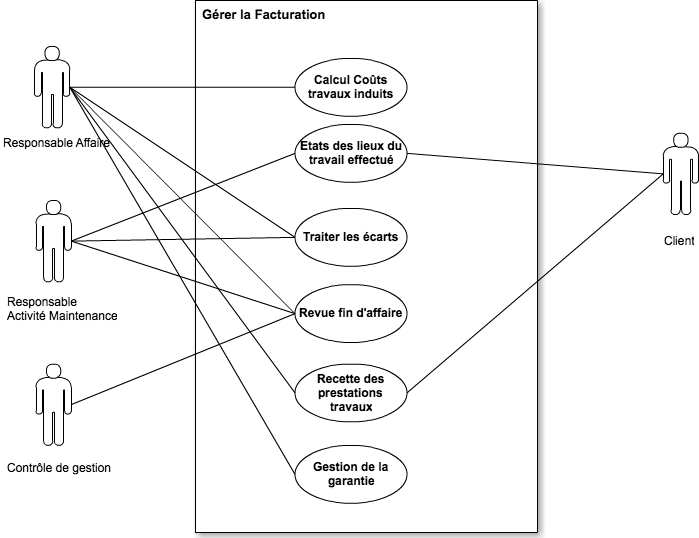
\includegraphics[width=\textwidth]{png/DCUGererFacturation.png}
\end {center}


\section{Définition des axes de progrès}

Les processus détaillés dans les documents annexes fonctionnent le plus souvent en parallèle et sur des applications informatiques différentes. Il en résulte que souvent les différentes unités organisationnelles ne sont pas en accord sur certains points. Le but principal de cette étude est donc de regrouper l'ensemble des procédures de gestion des contrats de maintenance au sein d'un même système d'information ou chaque unité organisationnelle aurait son rôle.

